\documentclass{article}
\usepackage{graphicx}
\usepackage{amsmath}

\title{Assessment of Pitch Estimation Algorithm pitchYinFFT for Single-note Instrument Sounds}
\author{Akke Houben}
\date{2016}

%\begin{figure}
%	\includegraphics{img/plan_tot.jpg}
%	\caption{Total plan of the system}
%	\label{fig:total}
%\end{figure}

\begin{document}
\maketitle

% --------------------------------------------------------------------------------------|
% Introduction
% --------------------------------------------------------------------------------------|
\section{Introduction}
Freesound\footnote{http://freesound.org/} is a project initiated and maintained by the Music Technology Group of the Universitat Pompeu Fabra (Barcelona) \footnote{http://mtg.upf.edu/} with the aim to "create a huge collaborative database of audio snippets, samples, recordings, bleeps, ... released under Creative Commons licenses that allow their reuse." and "to create an open database of sounds that can also be used for scientific rescearch and be integrated in third party applications." (http://freesound.org/). Following these aims efforts are undertaken to present the collection of sounds is multiple ways. This database contains a vast collection of single-note instrument sounds, which can be perfectly usable to use in software sample synthesisers to create digital instruments which are playable with for instance a MIDI keyboard. However it is a challenge to automatically collect the right sounds together and to make sure all the needed sounds are found or created. This current article will adres the problem of pitch estimation of single-note sounds. It is important to be able to get reliable pitch estimates as the software sample synthesiser demands that the rightly pitched sound is placed under the right keyboardkey. The Freesound pitch estimation is done using the pitchYinFFT algorithm contained in the Essentia library (Bogdanov, et al., 2013; http://essentia.upf.edu/). The pitchYinFFT is a optimalisation proposed by Brossier (Brossier, 2007) for reduced calculation time of the YIN algorithm of Cheveigné and Kawahara (Cheveigné & Kawahara, 2002; Bogdanov, et al., 2013). 
In this document the performance of the pitch estimation algorithm used by Freesound to estimate the pitches of sounds on single-note sounds will be assessed. The method used in this assessment is quite straight forward. A large collection of annotated sounds is gathered from Freesound and two other sources\footnote{Attached is a desription of the sounds used in this assessment as well as a comparison between the pitch estimates taken from Freesound and the locally computed estimates.}.
 This assessment will consist of a observation of the quality of the estimation (1), followed by a discussion on factors able to predict the quality of this estimation (2). Lastly possible improvements to the algorithm or the useage of the algorithm will be proposed and discussed (3).
% --------------------------------------------------------------------------------------|

% --------------------------------------------------------------------------------------|
% Performance of pitch estimation
% --------------------------------------------------------------------------------------|
\section{Performance of the pitch estimation}
\subsection{Method}
The performance of the pitch estimation algortihm will be assessed by comparing the pitch estimated by the algorithm against the pitch annotated for that sound, taken either from the filename or the descriptions and/or tags of the sounds. In this section the usage of the pitchYinFFT is the same as is implemented in Freesound. 
% /Method

\subsection{Results}
% /Results
Figure \ref{fig:pTag_distr} shows the distribution of the annotated pitches and figure \ref{fig:pEst_distr} shows the distribution of corresponding estimated pitches. The mean difference between the annotated and estimated pitches is $109Hz$ ($\sigma = 504.5Hz$). Around $58\%$ of the sounds are estimated higher than they are annotated. In table \ref{table:pTag_pEst} some statistical values of the annotated and estimated pitches are given.

\begin{figure}
    \centering
    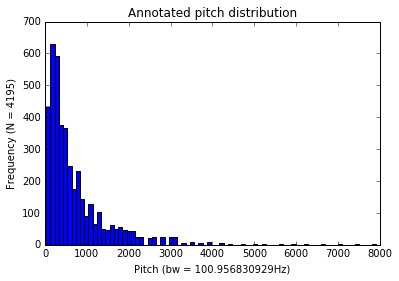
\includegraphics[scale=0.5]{img/pTag_distribution.png}
    \caption{Distribution of annotated pitches}
    \label{fig:pTag_distr}
\end{figure}
\begin{figure}
    \centering
    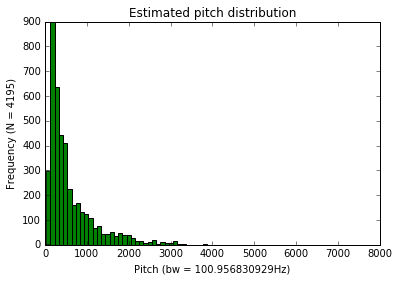
\includegraphics[scale=0.5]{img/pEst_distribution.png}
    \caption{Distribution of estimated pitches}
    \label{fig:pEst_distr}
\end{figure}
\begin{figure}
    \centering
    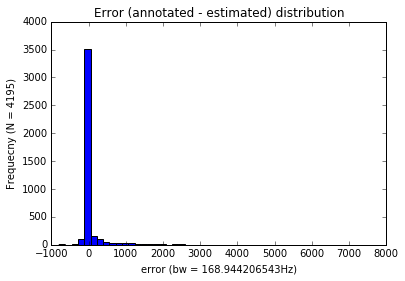
\includegraphics[scale=0.5]{img/err_distribution.png}
    \caption{Distribution of errors (annotation - estimation)}
    \label{fig:err_distr}
\end{figure}

\begin{table}[h]
    \begin{center}
        \begin{tabular}{ | l | c | c | r |}
            \hline
                        &   mean:       &   std:        &   median:     \\  \hline
            Annotated:  &   $711.7Hz$   &   $749.0Hz$   &   $440.0Hz$   \\  \hline
            Estimated:  &   $602.4Hz$   &   $584.2Hz$   &   $390.2Hz$   \\  
            \hline
        \end{tabular}
        \caption{Annotated and Estimated pitches}
        \label{table:pTag_pEst}
    \end{center}
\end{table}
As pitch is clearly a human percept it is more usefull not to talk in terms of frequencies, but some other scale. Below the error values are converted to Equivalent Rectangular Bandwidths and to semitones. In the rest of this document the semitone difference is used, as this is a in the scope of the current project an understandable and meaningfull measure. 

\begin{figure}
    \centering
    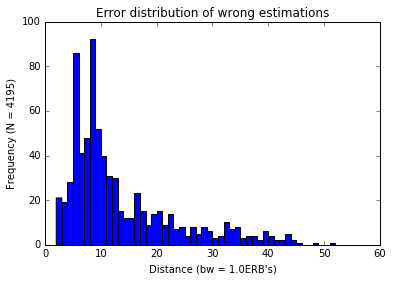
\includegraphics[scale=0.5]{img/erb_distribution.png}
    \caption{Distribution of ERB distances of wrong estimates}
    \label{fig:erb_distr}
\end{figure}

\begin{figure}
    \centering
    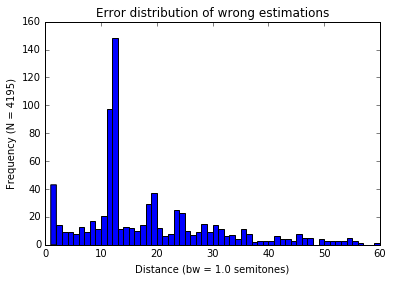
\includegraphics[scale=0.5]{img/st_distribution.png}
    \caption{Distribution of semitone distances of wrong estimates}
    \label{fig:st_distr}
\end{figure}

\begin{table}[h]
    \begin{center}
        \begin{tabular}{ | l | c | c | c || r |}
            \hline
                        &   mean:       &   std:        &   median:     &   $distance < 1$:\\  \hline
            ERBs:       &   $3.12ERBs$  &   $6.15ERBs$  &   $1.00ERBs$  &   $82.34\%$   \\  \hline
            semitones:  &   $3.58st$    &   $8.95st$    &   $0.12st$    &   $81.33\%$   \\  
            \hline
        \end{tabular}
        \caption{ERB and semiton distances}
        \label{table:ERB_st}
    \end{center}
\end{table}

From this point onward the estimations with a difference between the estimation and annotation of less than one semitone are called 'correct estimations'. Estimations with a difference bigger or equal to one semitone are called 'incorrect estimations'.

Figure \ref{fig:erb_distr} shows that around $82\%$ of the estimations fall within the same ERB as the annotated pitch and figure \ref{fig:st_distr} shows that $81\%$ of the estimations differ less than 1 semitone from the annotated pitch.

A common error in pitch estimations are ocatve errors (Gerhard, 2003), here the pitch is estimated to be a (sub) harmonic of the annotated pitch of the sound. Figure \ref{fig:st_distr} shows a clear peak in the bands corresponding to a distance of 12 semitones. Around $52.36\%$ of the errors can be identified as octave errors using the histogram of figure \ref{fig:octerr1}.

\begin{figure}
    \centering
    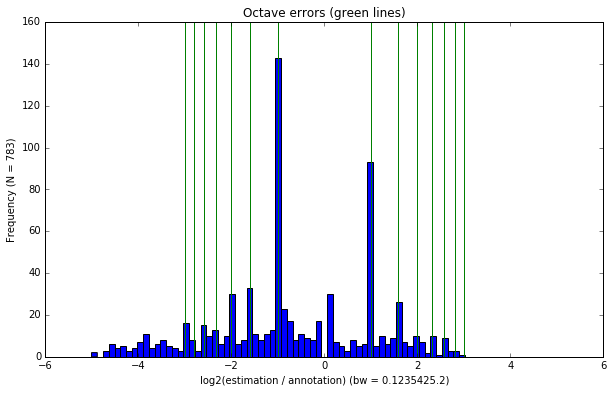
\includegraphics[scale=0.5]{img/octerr1.png}
    \caption{Octave Errors}
    \label{fig:octerr1}
\end{figure}

\subsection{Discussion}
As can be seen from figure \ref{fig:err_distr} most errors fall within a bandwidth close to 0Hz. However the mean of the point-wise errors is around 109Hz. Looking at the mean error and the mean and median values of the annotated versus the estimated pitches the pitch estimator tends to estimate pitches lower than the anntotation. However when the median value of the point-wise errors and the percentage of sounds with a higher annotation than estimation, suggest that there are some big differences where the estimation is cosiderably lower than the annotation. Also the median of the point-wise errors lies very close to 0Hz thus it can be inferred that no clear tendency to estimate too low or too high can be determined.

Figure \ref{fig:st_distr} and figure \ref{fig:octerr1} show that quite a lot of errors can be identified as octave errors. A clear improvement can be made by reducing the chance of octave errors occurring.
% --------------------------------------------------------------------------------------|

% --------------------------------------------------------------------------------------|
% Prediction of Errors
% --------------------------------------------------------------------------------------|
\section{Prediction of Errors}
In this section measurements to predict the performance of the estimation are investigated. Firstly predictors for the amplitude of the errors are looked at. After this factors which indicate the occurence of octave errors will be investigated.

\subsection{Method}
Several measurements will be investigated for their usefullness as predictors for the correctness of the estimates. Firstly some values returned by the pitchYinFFT and one measure directly related to the tonality of the signal are discussed. Secondly some other tonal and aural descriptors which can predict high error values are searched. The methods used to determine the usefullness of each measurement are fourfold:
\begin{enumerate}
    \item Firstly the difference in the mean of the values of the measurements between the correctly and incorrectly estimated sounds, the bigger this difference the more usefull the measurement. 
    \item Secondly the descriptors are tested for their abilities to correctly identify what sounds will be correctly estimated. The descriptors which acceptations and rejections coincide mostly with respectively the correctly and the incorrectly estimated sounds (highest percetage of true positives and true negatives) are most potent as predictors. 
    \item Lastly the 'Select Attributes' functionality from Weka (http://www.cs.waikato.ac.nz/ml/weka/) using as Attribute Evaluator the 'InfoGainAttributeEval' and as Search Method the 'Ranker' is used.
\end{enumerate}
When considering predictors for octave errors, octave errors are considered 'incorrect estimations' and all estimates which are no octave errors are considered 'correct estimations'

\subsubsection{Pitch estimation related}
The pitch estimator used returns a confidence measurement, this should be a measure for the quality of the estimation. Besides the confidence measure the variance of the pitch estimation for each sound could be a prediction for the quality of the estimation. The pitch estimation is combined with a pitch salience measurement. Salience is an indication for howmuch tonal information the signal contains and as the pitch estimator is designed for tonal sound this could also be a predictor for the size of the estimation errors.

\subsubsection{Descriptors}
Due to the characteristics of the algorithms used in the pitchYinFFT pitch estimation some type of sounds could be more difficult to be correctly estimated than others. In this section some descriptor values\footnote{Find attached a list of the calculated descriptors} are calculated for the sounds used in the pitch estimation. Correlations are investigated between the values obtained for the descriptors and the errors of the pitch estimation. 

\subsection{Results}
\subsubsection{Pitch estimation related}
\begin{figure}
    \centering
    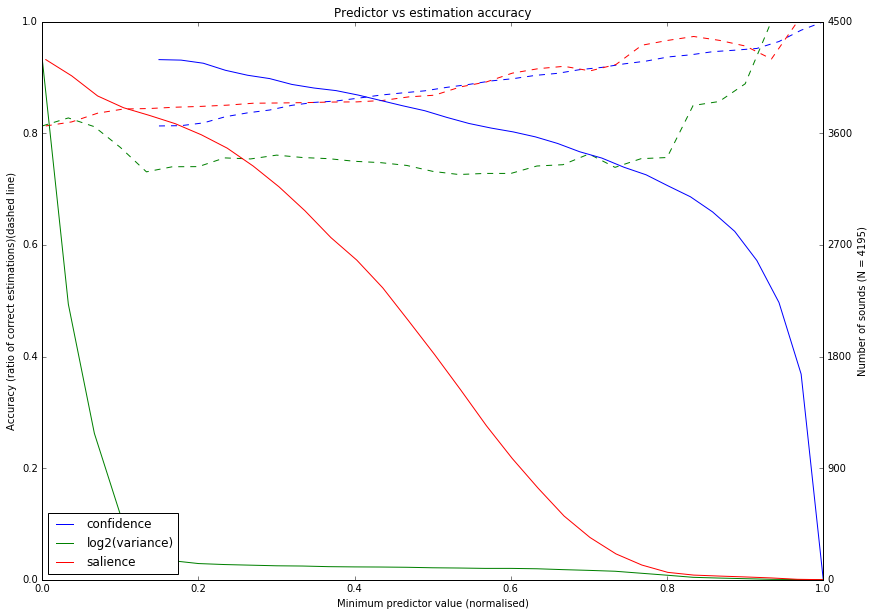
\includegraphics[scale=0.5]{img/penr_cvs.png}
    \caption{Precision and Recall of confidence, variance and salience}
    \label{fig:penr_cvs}
\end{figure}
In figure \ref{fig:penr_cvs} the precision and recall of the confidence, variance and salience can be seen. For each value of the predictor (confidence, variance or salience) an accuracy is calculated (ratio of correctly included versus total amount of accepted sounds). The variance is transformed to a standard deviation value by taking the square root of the variance, becuase this provided a more informative predictor.
\begin{table}[h]
    \begin{center}
        \begin{tabular}{ | l | l | c | c |}
            \hline
                        &           &   mean:       &   std:        \\ \hline
            Confidence  &           &               &               \\  \hline
                        & Correct:  &   $0.91424$   &   $0.13082$   \\  \hline
                        &Incorrect: &   $0.58102$   &   $0.25699$   \\  \hline
            Norm. diff.:    &   $0.33321$   &&\\  \hline
            \hline
            Variance:   &           &               &               \\  \hline
                        & Correct:  &   $-5.00515$  &   $1.74010$   \\  \hline
                        &Incorrect: &   $-4.95345$   &   $1.70110$   \\  \hline
            Norm. diff.:    &   $0.00441$   &&\\  \hline
            \hline
            Salience:   &           &               &               \\  \hline
                        & Correct:  &   $0.46339$   &   $0.19306$   \\  \hline
                        &Incorrect: &   $0.34857$   &   $0.21645$   \\  \hline
            Norm. diff.:    &   $0.11482$   &&\\  \hline
        \end{tabular}
        \caption{Difference in mean and std}
        \label{table:related}
    \end{center}
\end{table}
In table \ref{table:related} the difference in mean and standard deviationvalues between the correct and incorrect estimations are given.
\begin{table}[h]
    \begin{center}
        \begin{tabular}{ | l | r |}
            \hline
            Predictor:  &   Performance:\\  \hline
            \hline
            Confidence: &   $82.43\%$   \\  \hline
            Variance:   &   $54.61\%$   \\  \hline
            Salience:   &   $58.31\%$   \\  \hline
        \end{tabular}
        \caption{Discrimination Performance}
        \label{table:pred_cvs}
    \end{center}
\end{table}
Table \ref{table:pred_cvs} shows the performance of confidence, variance and salience in discriminating the correct from the incorrect estimations.
\begin{table}[h]
    \begin{center}
        \begin{tabular}{ | l | l |}
            \hline
            InfoGain:   &   Descriptor: \\  \hline
            \hline
            $0.4224$    &   Confidence  \\  \hline
            $0.1223$    &   Salience    \\  \hline
            $0.0115$    &   Variance    \\  \hline
        \end{tabular}
        \caption{WEKA Ranking of confidence, variance and salience}
        \label{table:weka_cvs}
    \end{center}
\end{table}
Lastly table \ref{table:weka_cvs} lists the ranking of the confidence, variance and salience found by WEKA, The correct results were sampled randomly \footnote{Find attached a document with a comparison of the sample and the total dataset}.

\begin{table}[h]
    \begin{center}
        \begin{tabular}{ | l | l | c | c |}
            \hline
                        &                   &   mean:       &   std:        \\ \hline
            Confidence  &                   &               &               \\  \hline
                        &Correct:           &   $0.91424$   &   $0.13082$   \\  \hline
                        &Octave errors:     &   $0.65720$   &   $0.24652$   \\  \hline
                        &Non-octave errors: &   $0.50202$   &   $0.24590$   \\  \hline
            \hline
            Variance   &                    &               &               \\  \hline
                        &Correct:           &   $0.61659$   &   $0.13330$   \\  \hline
                        &Octave errors:     &   $0.61698$   &   $0.14706$   \\  \hline
                        &Non-octave errors: &   $0.63779$   &   $0.11131$   \\  \hline
 
           Salience   &                     &               &               \\  \hline
                        &Correct:           &   $0.46339$   &   $0.19306$   \\  \hline
                        &Octave errors:     &   $0.46938$   &   $0.46938$   \\  \hline
                        &Non-octave errors: &   $0.32663$   &   $0.24057$   \\  \hline
        \end{tabular}
        \caption{Difference in mean and std (octave errors)}
        \label{table:msdiffOct_cvs}
    \end{center}
\end{table}
In table \ref{table:msdiffOct_cvs} the difference in mean and standard deviationvalues between the correct, the incorrect attributable to octave errors and non-octave error incorrect estimations are given. 

\subsubsection{Descriptors}
\begin{figure}
    \centering
    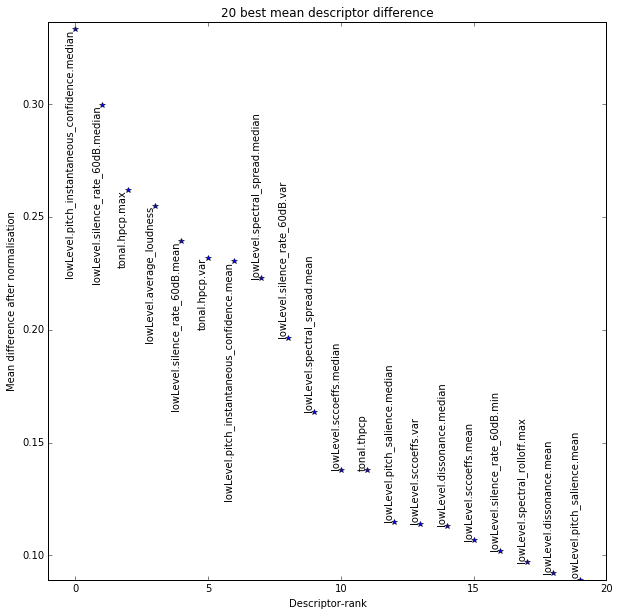
\includegraphics[scale=0.5]{img/pred_descr.png}
    \caption{Difference in mean values}
    \label{fig:pred_desc}
\end{figure}
Figure \ref{fig:pred_desc} shows the twenty descriptors with the biggest difference in mean value between the correct and incorrect estimations. 
\begin{figure}
    \centering
    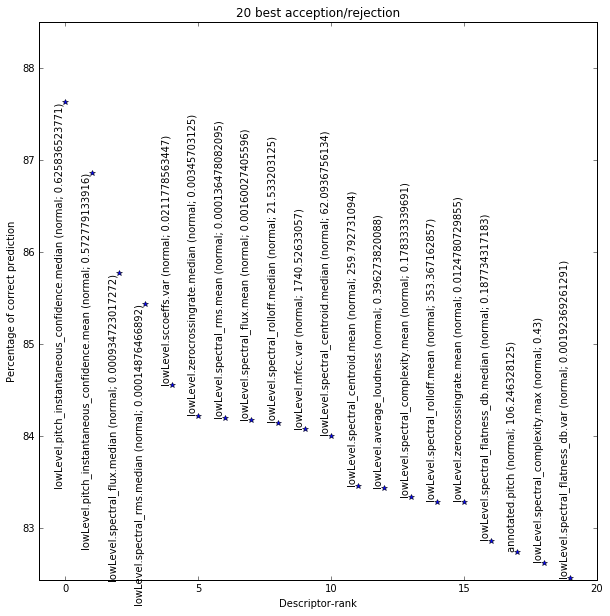
\includegraphics[scale=0.5]{img/pn_descr.png}
    \caption{Discriminate correct from incorrect}
    \label{fig:pn_desc}
\end{figure}
 The twenty best descriptors to divide the estimations into correct and incorrect estimations are given in figure \ref{fig:pn_desc}, also the treshold is given for the descriptor under consideration.
\begin{table}[h]
    \begin{center}
        \begin{tabular}{ | l | l |}
            \hline
            InfoGain:   &   Descriptor: \\  \hline
            \hline
            $0.423139$  &   lowLevel.pitch\_instantaneous\_confidence.median \\ \hline
            $0.374362$  &   lowLevel.pitch\_instantaneous\_confidence.mean \\ \hline
            $0.284290$  &   lowLevel.spectral\_spread.median    \\  \hline
            $0.185515$  &   lowLevel.spectral\_spread.mean    \\  \hline
            $0.148130$  &   lowLevel.spectral\_skewness.median    \\  \hline
            $0.132967$  &   lowLevel.spectral\_rolloff.mean    \\  \hline
            $0.128956$  &   lowLevel.spectral\_flatness\_db.median    \\  \hline
            $0.127023$  &   lowLevel.average\_loudness    \\  \hline
            $0.124936$  &   sfx.pitch\_min\_to\_total    \\  \hline
            $0.123078$  &   lowLevel.spectral\_centroid.mean    \\  \hline
            $0.121924$  &   lowLevel.silence\_rate\_60dB.mean    \\  \hline
            $0.110486$  &   lowLevel.pitch.median    \\  \hline
            $0.110434$  &   lowLevel.spectral\_rms.median    \\  \hline
            $0.101883$  &   lowLevel.dissonance.median    \\  \hline
            $0.098656$  &   lowLevel.barkbands\_skewness.mean    \\  \hline
            $0.096012$  &   lowLevel.spectral\_rms.mean    \\  \hline
            $0.095506$  &   lowLevel.barkbands\_skewness.median    \\  \hline
            $0.093984$  &   lowLevel.pitch\_salience.median    \\  \hline
            $0.091919$  &   lowLevel.spectral\_complexity.mean    \\  \hline
            $0.091475$  &   lowLevel.spectral\_strongpeak.median    \\  \hline
        \end{tabular}
        \caption{WEKA Ranking of descriptors}
        \label{table:weka_desc}
    \end{center}
\end{table}
Table \ref{table:weka_desc} lists the descriptors from most usefull to classify incorrect and correct estimations to the less usefull.
\begin{figure}
    \centering
    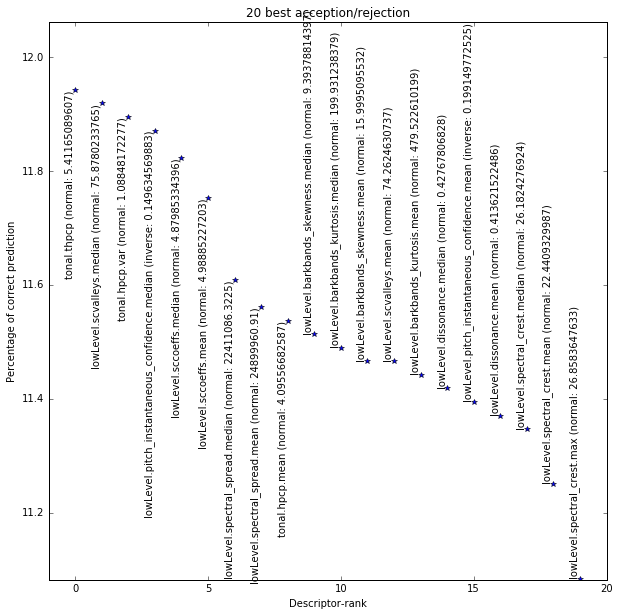
\includegraphics[scale=0.5]{img/pnOct_descr.png}
    \caption{Discriminate octave errors}
    \label{fig:pnOct_desc}
\end{figure}
Figure \ref{fig:pnOct_desc} lists the twenty best descriptors to classify the octave errors from the other estimations, also the tresholds are given.
\begin{table}[h]
    \begin{center}
        \begin{tabular}{ | l | l |}
            \hline
            InfoGain:   &   Descriptor: \\  \hline
            \hline
            $0.296336$  &   lowLevel.pitch\_instantaneous\_confidence.mean   \\ \hline
            $0.250393$  &   lowLevel.pitch\_instantaneous\_confidence.median   \\ \hline
            $0.200927$  &   lowLevel.spectral\_spread.median   \\ \hline
            $0.145147$  &   lowLevel.spectral\_skewness.median   \\ \hline
            $0.144761$  &   lowLevel.spectral\_spread.mean   \\ \hline
            $0.141825$  &   lowLevel.silence\_rate\_60dB.mean   \\ \hline
            $0.141121$  &   lowLevel.spectral\_flatness\_db.median   \\ \hline
            $0.130088$  &   lowLevel.spectral\_complexity.mean   \\ \hline
            $0.127021$  &   lowLevel.spectral\_complexity.median   \\ \hline
            $0.122647$  &   lowLevel.spectral\_rms.median   \\ \hline
            $0.117874$  &   sfx.pitch\_min\_to\_total   \\ \hline
            $0.115669$  &   lowLevel.spectral\_flatness\_db.mean   \\ \hline
            $0.114153$  &   lowLevel.spectral\_rms.mean   \\ \hline
            $0.105331$  &   lowLevel.barkbands\_skewness.mean   \\ \hline
            $0.104639$  &   lowLevel.spectral\_energyband\_middle\_high.median   \\ \hline
            $0.094725$  &   lowLevel.spectral\_kurtosis.median   \\ \hline
            $0.094578$  &   lowLevel.barkbands\_spread.median   \\ \hline
            $0.091152$  &   lowLevel.spectral\_rolloff.mean   \\ \hline
            $0.090370$  &   lowLevel.spectral\_rolloff.median   \\ \hline
            $0.086788$  &   lowLevel.dissonance.mean   \\ \hline

       \end{tabular}
        \caption{WEKA Ranking of descriptors for octave errors}
        \label{table:wekaOct_desc}
    \end{center}
\end{table}
The ranking of the descriptors to classify the estimations between those which are octave errors and which are not, obtained trough WEAK is given in table \ref{table:wekaOct_desc}.

\subsection{Discussion}
\subsubsection{Pitch estimation related}
It is visible from figure \ref{fig:penr_cvs}  that the confidence, variance and salience perform equally well with a low minimal predictor value. However the confidence measurement clearly outperforms the other with a higher minimal value both in terms of sounds included without suffering a loss in accuracy. Tables \ref{table:pred_cvs} and \ref{table:weka_cvs} also show that the confidence is the most usefull to discriminate the correct from the incorrect estimations. 
The confidence measurement also seems to be the best in discriminating octave errors from non-octave errors, but to a lesser extend.

\subsubsection{Descriptors}
In the above data the earlier observation that the 'confidence' measurement was a good prediction for the errors is confirmed. Also the salience and pitch variance measurements again seem to be able to predict the error values to some extend. 
From figure \ref{fig:pred_desc} and especially figure \ref{fig:pn_desc} a clear importance can be seen of the 'silence\_rate' descriptors. These descriptors give a measure for the ammount frames with a signal above a certain amplitude treshold versus the amount of frames with a signal below a certain amplitude treshold. Also figure \ref{fig:pred_desc} indicates that the 'average\_loudness' is a descriptor that is able to predict a lot of errors, this measurement is ofcourse influenced by the presence of silent frames, but it is also possible that some sounds are very silent and in this way badly influence the estimation.
Quite a few descriptors relating to the spectral characteristics of the sounds are identified as important in separating the right from wrong estimations. The descriptors containing 'spectral' in the name; the descriptors 'sccoeffs' and 'scvallets' and; all the descriptors with 'barkbands' are measurements of the spectral characteristics of the sounds. The 'sccoeffs' and 'scvalleys' relate to the contrast between the spectral peaks and the spectral valleys. The 'spectral' descriptors measure different characteristics of the spectral distribution. The 'barkbands' use a different frequency scale (a Bark band scale instead of a linear frequency scale). Spectral skewness relates to the asymetry of the spectrum. Spectral kurtosis is a measurement for the tailedness (amount of 'outliers') of the spectrum. In addition to these the 'dissonance' and 'oddtoevenharmonicenergyratio' descriptors give information about the content and makeup of the tonal material in the signal. 
Lastly a few descriptors relating to the pitch of the sounds are identified as usefull to select the sounds which will result in high errors in the pitch estimation. The 'hpcp' and 'thpcp' descriptors relate to the note (pitch class) of the signal irrespective of the octave it is in. The values from the 'hpcp' descriptor that are important to separate the correct from the incorrect estimations is the variance and maximal value of the hpcp per sound. If the hpcp value varies alot througout a sound the algorithm is not finding the same pitch class for succesive frames of a sound. The 'thpcp' calculates the relative intensity of all the 12 pitches in the western diatonic pitch system. However in this calculation the vector returned by the descriptor is summed to obtain a single value to use to separate the estimations. A higher value thus corresponds to one pitch being relatively more present than the other pitches, during the sound. The prominence of one pitch relative to the other pitches obviously relates to the 'ease' with which the pitch estimation algorithm can find the pitch, as the pitch is more prominent. Interestingly the Weka ranker also finds the 'pitch.median' measurement (the estimated pitch) valuable to discriminate the sounds as visible in table \ref{table:weka_desc}.

Also for the identification of the octave errors the confidence measurement seems a usefull separator, however the difference is not so big. Also again the 'silence\_rate' seems to influence the estimation, but again it is not very reliable. Basically, the measurements which predict errors or separate errors from non-errors are also able to predict and separate octave errors altough -unfortunately- to a lesser extend. 
% --------------------------------------------------------------------------------------|

% --------------------------------------------------------------------------------------|
% Improvements
% --------------------------------------------------------------------------------------|
\section{Improvements}
In the following section the results obtained in the above steps are discussed to propose improvements to the pitch estimation. The improvements can be based on one hand on identification of erroneous estimations and discarting these from the pool or recalculating the estimation with different parameters or implementations. On the other hand the some improvements are proposed to increase the accuracy of the estimations.



% --------------------------------------------------------------------------------------|

% --------------------------------------------------------------------------------------|
% Conclusion
% --------------------------------------------------------------------------------------|
\section{Conclusion}
% --------------------------------------------------------------------------------------|

% --------------------------------------------------------------------------------------|
% References
% --------------------------------------------------------------------------------------|


\section{References}

\end{document}
